%!TEX root = ChapSpringer_Main.tex
\subsection{Implementation}
In order to assess physical parameters of an Integrated Circuit (IC) we need to create an IC layout model. In traditional IC design this model is typically generated after gate-level synthesis and place\&route (P\&R). Both steps are performed using Electronic Design Automation (EDA) tools, in a sequence of many different tools. The whole processes typically requires many man and CPU cycles before final model is built. This is due to the system complexity; the accuracy of the models at different abstraction levels that we need to build; and the lack of completely automated methods and algorithms (most of the problems that any design flow is solving are NP-hard problems). To deal with 3D design we have extended the commercially available tools suite from Atrenta (now Synopsis). 

The flow is depicted on Figure~\ref{fig:3DFlow}, and we do provide a bit more detailed explanation of each flow step.

\begin{figure}[!b]%
\centering
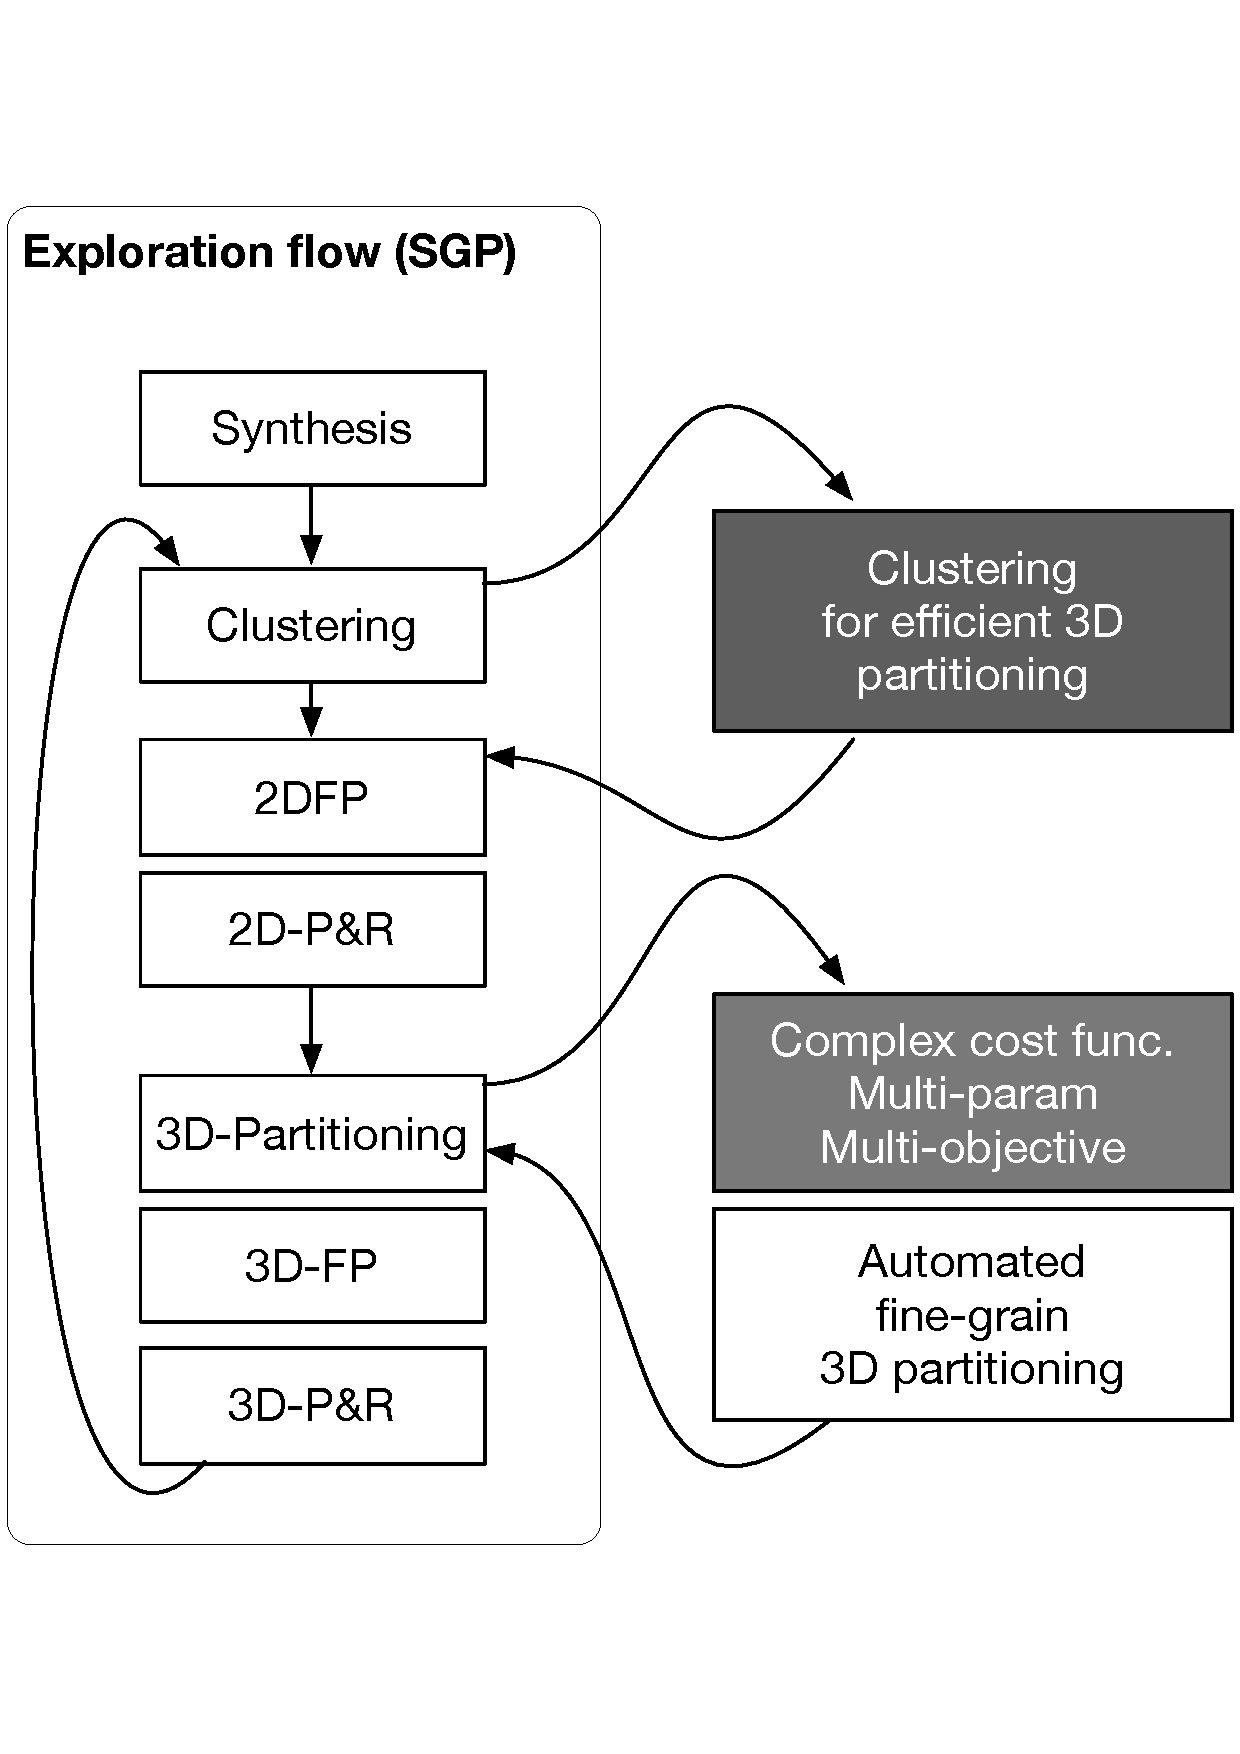
\includegraphics[width=0.75\columnwidth]{DesignFlow.pdf}
\caption{Sequence of steps required to enable 3D-SIC design (3D Design Flow)\label{fig:3DFlow}}
\end{figure}

\textbf{Step 1: RTL Synthesis} – The input of the proposed flow, as in any IC design flow, consists of several elements. First we need to provide the description of the circuit itself. This is done using any of the standard Hardware Description Languages (VHDL, Verilog). Also, if present, abstracted high-level models of certain blocks cab be supplied with interface definition, area, power, timing etc. (i.e. black-boxes). Finally, typical system constraints (timing) are supplied through standardized file format (.sdc files). 

Once the design database is ready, the RTL is synthesized to gate-level netlist using standard technology files (.lib and .lef files) provided by the technology vendor. Note that if the design is intended for 2.5D/3D integration, the technology files will have to capture both electrical and geometrical information not only for standard cells, but also for 3D specific features such as TSVs, micro-bumps, Cu-pads, RDLs, etc. that will be instantiated depending on the stack configuration (F2F or F2B) chosen.

Synthesized gate-level netlist is analyzed for area, timing, logical congestion and other properties. The constraints and synthesis tool guides are adapted to reach realistic goals. Once the synthesis flow is stable i.e. the synthesis process produces the netlist in line with timing constraints, generated netlist can be used as input for both 2D and 3D physical design flows.

\textbf{Step 2: Clustering} – Prior to floorplanning, the gate-level netlist is partitioned into a number of  “reasonably” sized physical clusters of standard cells. The clustering is done so that the floorplan engine works on a reduced number of placeble instances. The size of clusters (the meaning of “reasonable”) will depend on the total circuit size. In general it is chosen in such a way, so that the total number of clusters is in order of few dozens to few hundreds of physical (thus placeble) entities. This is the optimal number of instances (tool run-time vs. quality of the solution) for the floorplan engine.

The purpose of this step is twofold. First, the system is viewed as an assembly of blocks, rather then a collection of logic gates (it could be few dozen of millions) in the design to enable floorplanning (i.e. block level placement) as explained. But secondly, such system view will help in establishing what should go where in the stack. 

Standard cell clustering can be performed using many different methods. Note that this is a very important step since the quality of the physical design will depend on the clustering scheme adopted. In the current design flow we can use either top-down approach (from top-level of the design, way to the standard cell level) or bottom-up (from the standard cell level and up). Different clustering objectives could be achieved during clustering: keeping and following the logical hierarchy, creating clusters of the similar size, hierarchical min-cut across the clusters, etc. Note that in the case of the 3D integration, the clustered netlist is further partitioned into a number of gate-level entities (that will remain clustered), equal to the number of dies in the system (see next step, 3D-Partitioning). 

\textbf{Step 3: 3D-Partitioning} – This step is performed only in a 3D flow. The stack structure: the number of dies, technology node on per die basis (this is to support heterogeneous integration), stacking orientation (face-up or face-down), 3D structure properties (TSV/ubump/CuPad) and RDL net properties (width/pitch), etc. are specified in a manually generated XML file, given as an input to the tool. The actual 3D partitioning of the gate level netlist is carried out in an automated fashion, using the stack configuration file, synthesized gate-level netlist. 

For 2.5 and 3D designs, the synthesized gate-level netlist is partitioned into so many gate-level entities as there are dies in the system. Depending on the 3D integration scheme appropriate inter-die interconnect models are applied. To enable the partitioning, the designer first needs to specify the initial stack structure. This is done with a manually created XML file. The stack is divided into tiers, each tier can contain multiple dies (all dies in the same tier have the same z coordinate). XML specifies also the orientation of each die in the stack (face-up or face-down). Each die container can also define its own TSV, micro-bumps, RDL properties that will override those specified in the technology file. This is to insure that during design exploration phase we can easily replace one basic technology parameter and understand the impact on the system performance (e.g. TSV size, form factor/pitch).

\begin{itemize}
\item User specified partitioning directives and
\item Automated partitioning 
\end{itemize}

In the case of user specified partitioning directives, the information on which block should go where is provided manually in the form of explicit block-to-die assignment directives using a dedicated tool command. However in of fine pitch 3D interconnects we could perform fine grain partitioning, i.e. system blocks are smaller and smaller. Thus their number, as well as their interconnectivity view, will increase considerably making manual partitioning process impossible.

In order to automate the partitioning we use graph theory, already extensively used in the field of the VLSI design. Graph structure, with vertex and edge mimic perfectly well a logic circuit, no meter the level of hierarchy we are looking at (although it might become very complex as we go down in the logical hierarchy). Graph vertex represents a logic gate or a cluster of standard cells (whatever the size of that cluster in terms of gates might be). The edge models the connection(s) between the gates (or clusters).

One of the particular problems that have been extensively covered in the graph theory literature concerns graph partitioning problem. For this problem the algorithm tries to automatically produce two, or eventually more graph partitions that have specific properties. Most of the time these properties aim certain cut objective: like min-cut, in which the sum of the weights of the cut edges is minimal. This can be eventually combined with the objective on vertexes that could be equally balanced between the partitions.

Graph partitioning is illustrated in Figure 12 where we show a simple graph with both edges and vertexes being weighted (the numbers between the square brackets). The initial graph, shown on the left is partitioned into two partitions, providing a min-cut on the edges (cut cost of 5) and balanced vertex weights (respectively the cost of 12 and 11 for Die0 and Die1).

\begin{figure}[!b]%
\centering
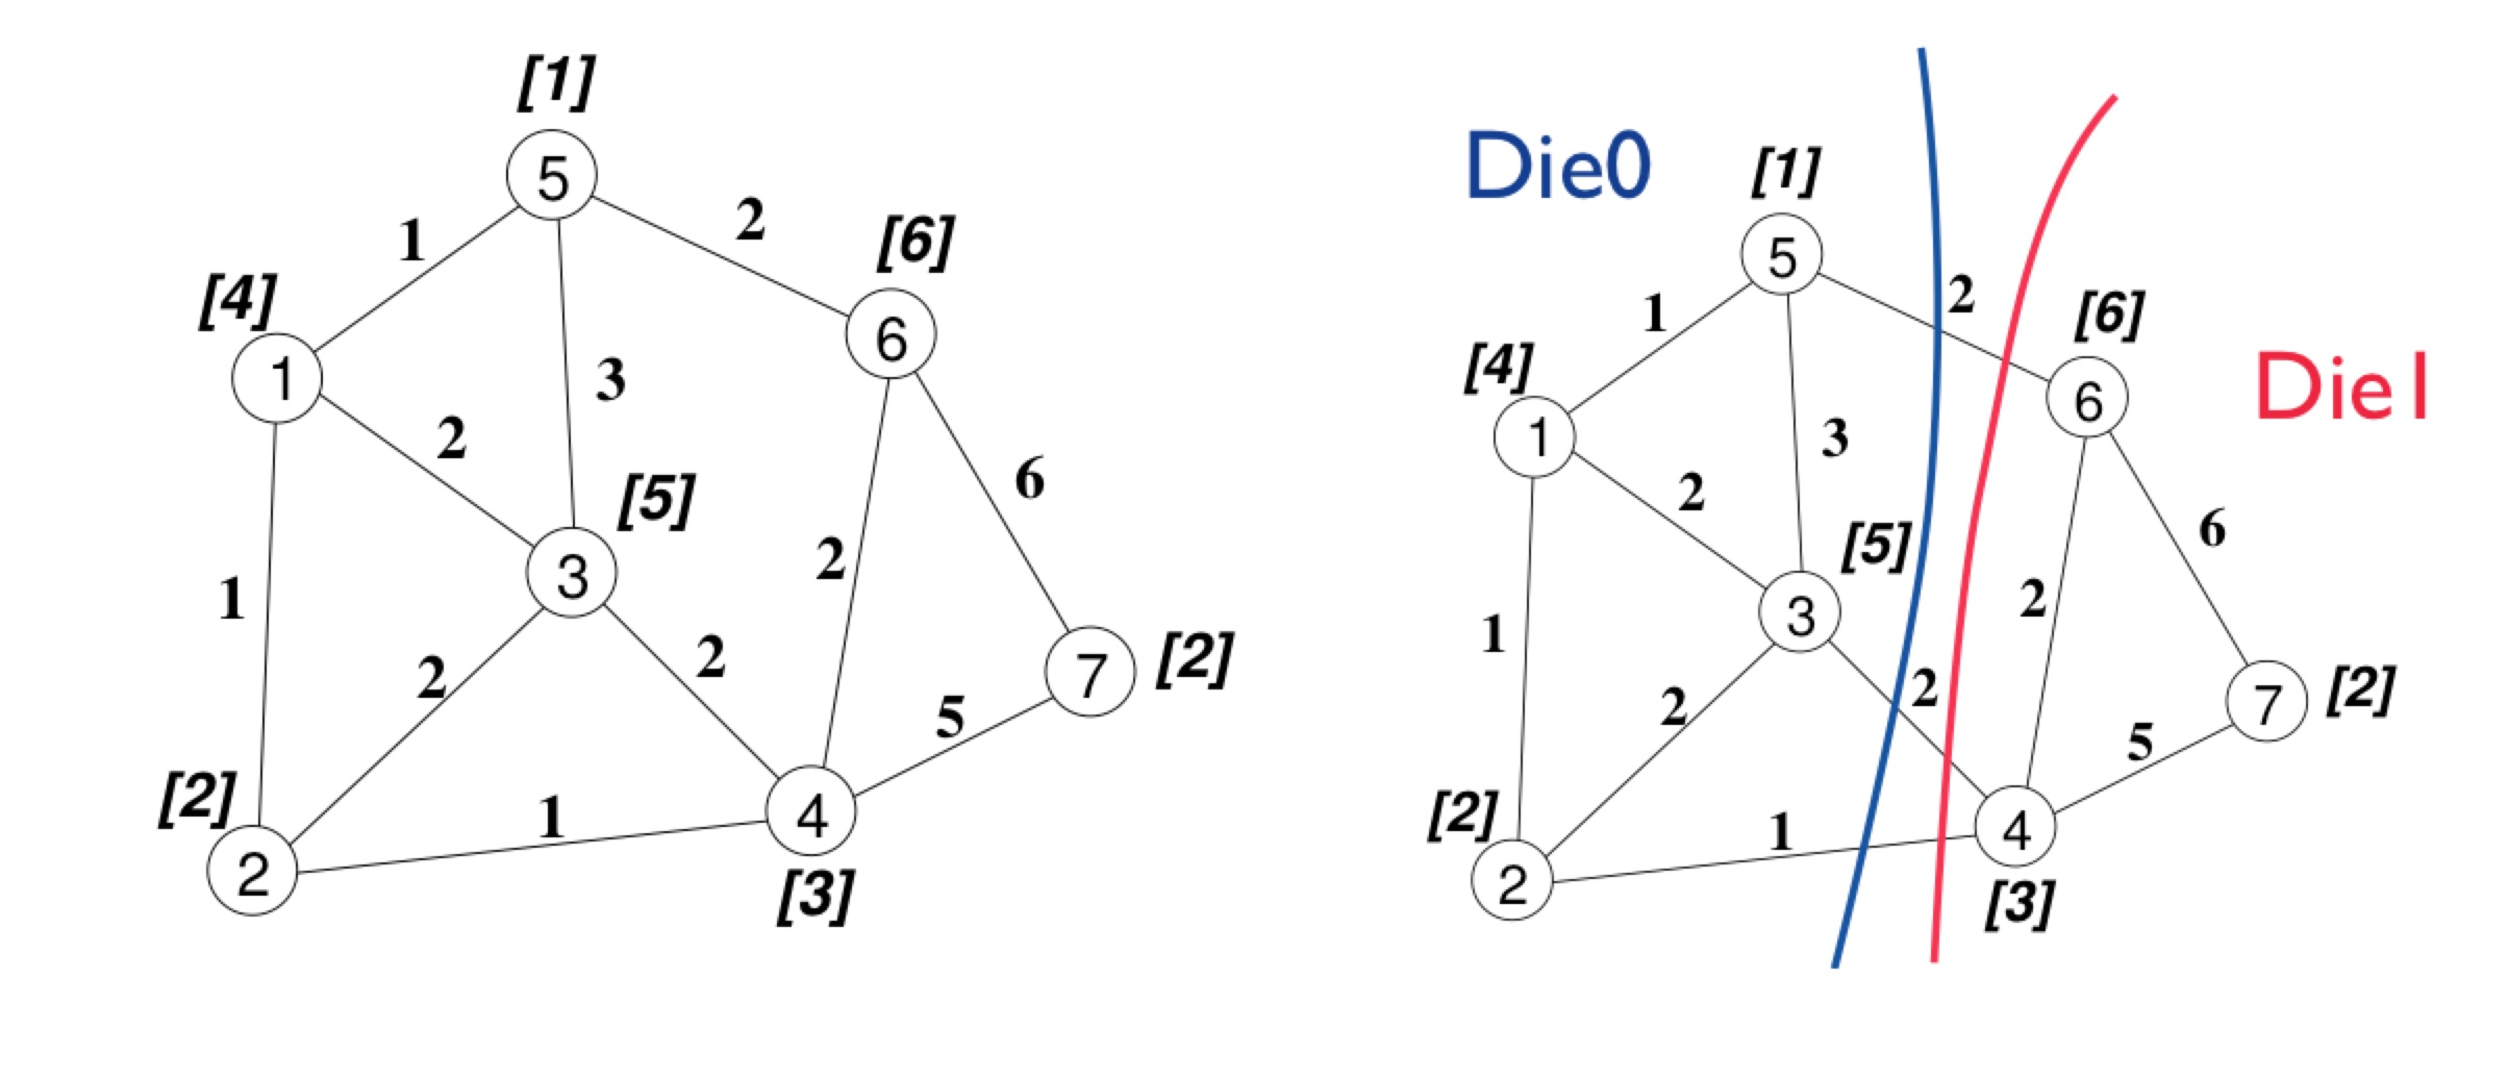
\includegraphics[width=0.95\columnwidth]{GraphPart.pdf}
\caption{Simple graph with annotated vertices (system blocks and their area) and edges ()\label{fig:GraphPart}}
\end{figure}

Once the partitioning information is generated (manually or automatically) the design is effectively partitioned. The tool performs module assignment for a given tier. During this process all inter die nets will be automatically extracted and corresponding physical inter-die net models applied depending on the die orientations (choice between F2F and F2B) and specified technology options. With internally partitioned netlist we can now proceed with floorplanning of the design, and this is then followed by standard cell placement and routing. At this stage the approximated layout of the circuit is generated and it can be characterized to assess system performance. Typically we extract area, congestion and timing analysis, power dissipation per component etc.

\textbf{Step 4: Floorplanning} – The clustering and 3D partitioning steps are followed by the floorplanning step. In case of 2D, the floorplanning is carried out automatically, with physical constraints that are manually generated based on connectivity analysis and whatever knowledge/constraints we might have on the design (e.g. hard-macro pre-placements etc.). In case of 3D, additional physical constraints related to 3D net placement are generated (TSV/micro-bump clustering and placement). Floorplanning is carried out for each die separately. Becasue 

\textbf{Step 5: Standard cell Placement and Routing (PNR)} – Standard cell placement and routing are carried out after floorplanning. In case of 3D, it is performed separately for each die, in a sequential fashion.
